\chapter{Scenarios and use cases}
\label{ch:scenarios}

\section{User related scenarios}
\newcommand{\see}[1][reference missing]{(see \specref{#1})}
The buttons and the yellow border in scenario 1 to 4 are specified in \ref{sec:sm_userinterface}.

\subsection{Scenario 1: User successfully records a session}
\begin{enumerate}
    \item The application displays a button at the bottom right corner of the screen.
    \item \Gls{user} clicks the button to start recording.
    \item The application starts to record and displays a yellow border on screen during the whole recording time to indicate that the \gls{session} is being recorded.
    \item \Gls{user} researches in different databases during recording.
    \item \Gls{user} finishes the research and clicks the same button to stop recording.
    \item The application displays a dialog to ask the \gls{user}, if the recording data should be saved or not.
    \item \Gls{user} clicks "save" to save the recorded data.
    \item The application saves the recorded data and the yellow border disappears at the same time.
\end{enumerate}

\subsection{Scenario 2: User discards a session}
\begin{enumerate}
    \item The application displays a button at the bottom right corner of the screen.
    \item \Gls{user} clicks the button to start recording.
    \item The application starts to record and displays a yellow border on screen during the whole recording time to indicate that the \gls{session} is being recorded.
    \item \Gls{user} is interrupted by multiple received Emails and reads the Emails for a long period of time.
    \item \Gls{user} realizes that the research only takes up 10\% of the total recording time and gives up on recording by clicking the same button.
    \item The application displays a dialog to ask the \gls{user}, if the recording data should be saved or not.
    \item \Gls{user} clicks "discard" and confirms their decision in the following dialog by clicking "Delete anyway" to discard the recorded data.
    \item The application discards the recorded data and the yellow border disappears at the same time.
\end{enumerate}

\setcounter{subsection}{3} %%removed section 9.1.3
\setcounter{subsection}{4} %%removed section 9.1.4

\setcounter{section}{2} %% removed section 9.2

\section{Administrator related scenarios}
\subsection{Scenario 6: Administrator changes configuration}
\begin{enumerate}
    \item The \gls{admin} opens the configuration file provided by the application.
    \item The \gls{admin} changes the enabled modules by editing the configuration file and saving it.
    \item The \gls{admin} distributes the changed configuration file to a \gls{user}.
    \item The \gls{user}'s application receives the changed configuration file .
    \item The enabled modules of the application is changed according to the received configuration file.
\end{enumerate}

\section{Use cases}
\begin{center}
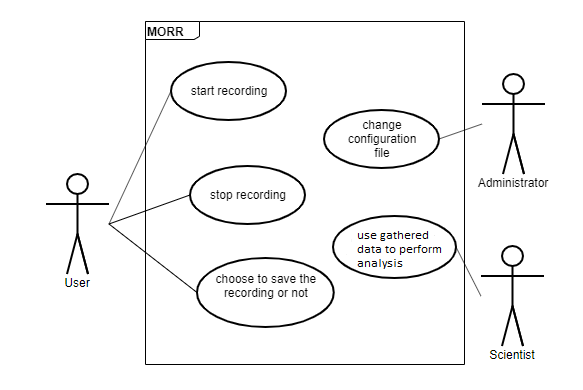
\includegraphics[scale=0.9]{resources/usecase.png}
\end{center}